\chapter{Research Results}
\begin{multicols}{2}
      \section{Introduction}
      This chapter presents the results of the research conducted to answer the research questions. The chapter is
      divided into two sections, each corresponding to one of the research questions. The first section presents
      the results of the research conducted to answer the first research question, while the second section
      presents the results of the research conducted to answer the second research question.

      \section{Research Sub-Question \#1: What is the current state of the QaaS app?}

      The \acrshort{qaas} app is an \gls{ERP} web application that is used by \acrshort{qict} and its clients.
      For \acrshort{qict}'s clients, it is a \acrshort{saas} that is used to
      For \acrshort{qict} employees themselves, it is an \acrshort{erp} system that is used to manage the clients and their
      \acrshort{ict} infrastructure. It is made in Dart with Flutter as the front-end framework. There are 2 main parts of the
      \acrshort{qaas} app, the front-end and the back-end. The front-end is made in Flutter, and the back-end is made in Node.js with
      TypeScript as the template. The back-end is hosted on Firebase Cloud Functions which are used to connect and make \acrshort{http}
      calls to the internal \acrshort{api}s, and the front-end is hosted on Firebase Hosting.

      \subsubsection{APIs and Technologies}
      The \acrshort{qaas} app also utilizes several \acrshort{api}s and technologies to help with its operations.
      It needs to manage and make connection different sort of \acrshort{api}s to help with the operations of the
      \acrshort{erp} application. Those \acrshort{api}s are the following:
      \begin{itemize}
            \item Resello: is used for \acrshort{qict} \acrshort{ms} subscriptions owned by Pax8 (\textit{\cite{resello}}).
                  It is a cloud marketplace that simplifies the way \acrshort{sme}s buy, sell, and manage cloud solutions
                  through automation. It provides a single platform to manage the entire cloud customer lifecycle, from
                  quote to cash to support, thus simplifying the process of buying, selling and managing cloud
                  solutions. Furthermore, it normally uses \gls{SOAP API} for its communication.
            \item SnelStart: is used for \acrshort{qict} automation of financial and accounting system software,
                  such as managing invoices, \acrshort{etc} for \acrshort{sme}s. It offers a range of products and
                  services to help businesses manage their finances, including accounting software, invoicing software,
                  and financial management tools.
            \item Bodyguard.io: is a \acrshort{cdr} tool used for security tab. It is a product from a Dutch company
                  that filters and scrutinizes downloads from web browsers to detect and prevent malicious files with
                  real-time download scanning capabilities. It normally uses \gls{RESTful API} for its
                  communication.
            \item N-Central: is a product from N-Able and is used for monitoring clients' devices and ensuring the
                  overall security of their systems, \acrshort{it} infrastructure, and digital assets. It is a
                  \gls{RMM} platform designed to help \acrshort{msp} and \acrshort{it} professionals to
                  remotely monitor and manage their clients' devices and networks. It provides a comprehensive
                  set of tools and features for monitoring, managing, and securing clients' devices and networks,
                  including remote monitoring and management, patch management, antivirus, backup and disaster
                  recovery, and network topology mapping. The return response from this \acrshort{api} is in \gls{XML}
                  and \acrshort{json} format, making it both a \gls{REST gls} and \acrshort{soap} \acrshort{api}.
            \item PerfectView: is used for \gls{CRM} software (\textit{\cite{perfectView}}). It is designed to
                  improve business relationships with customers, assist in customer retention, and drive sales growth.
                  In the \acrshort{qaas} app, it is used to manage the relationships and interactions with the app's users,
                  which could include tracking user interactions, managing customer support requests, and analyzing user
                  data to improve the app's functionality and \acrshort{ux}.
      \end{itemize}

      Besides all the 5 internal \acrshort{api}s that \acrshort{qict} uses, the company also uses several technologies to help them with their
      operations. Those tools are:

      \begin{itemize}
            \item Computicate (now newly named Acronis): is used as their ticketing system, providing ticketing solution services to customers for
                  a wide range of events and activities (\textit{\cite{computicate}}).
            \item TOMTelecom: is used for their company's phone system. It is responsible for structured process of call routing on incoming calls
                  from customers to the appropriate department or individuals, ensuring effective communication and issue resolution
                  (\textit{\cite{tomTelecom}}).
      \end{itemize}

      \subsection{The QaaS App Infrastructure}
\end{multicols}

\begin{figure}[htbp]
      \centering
      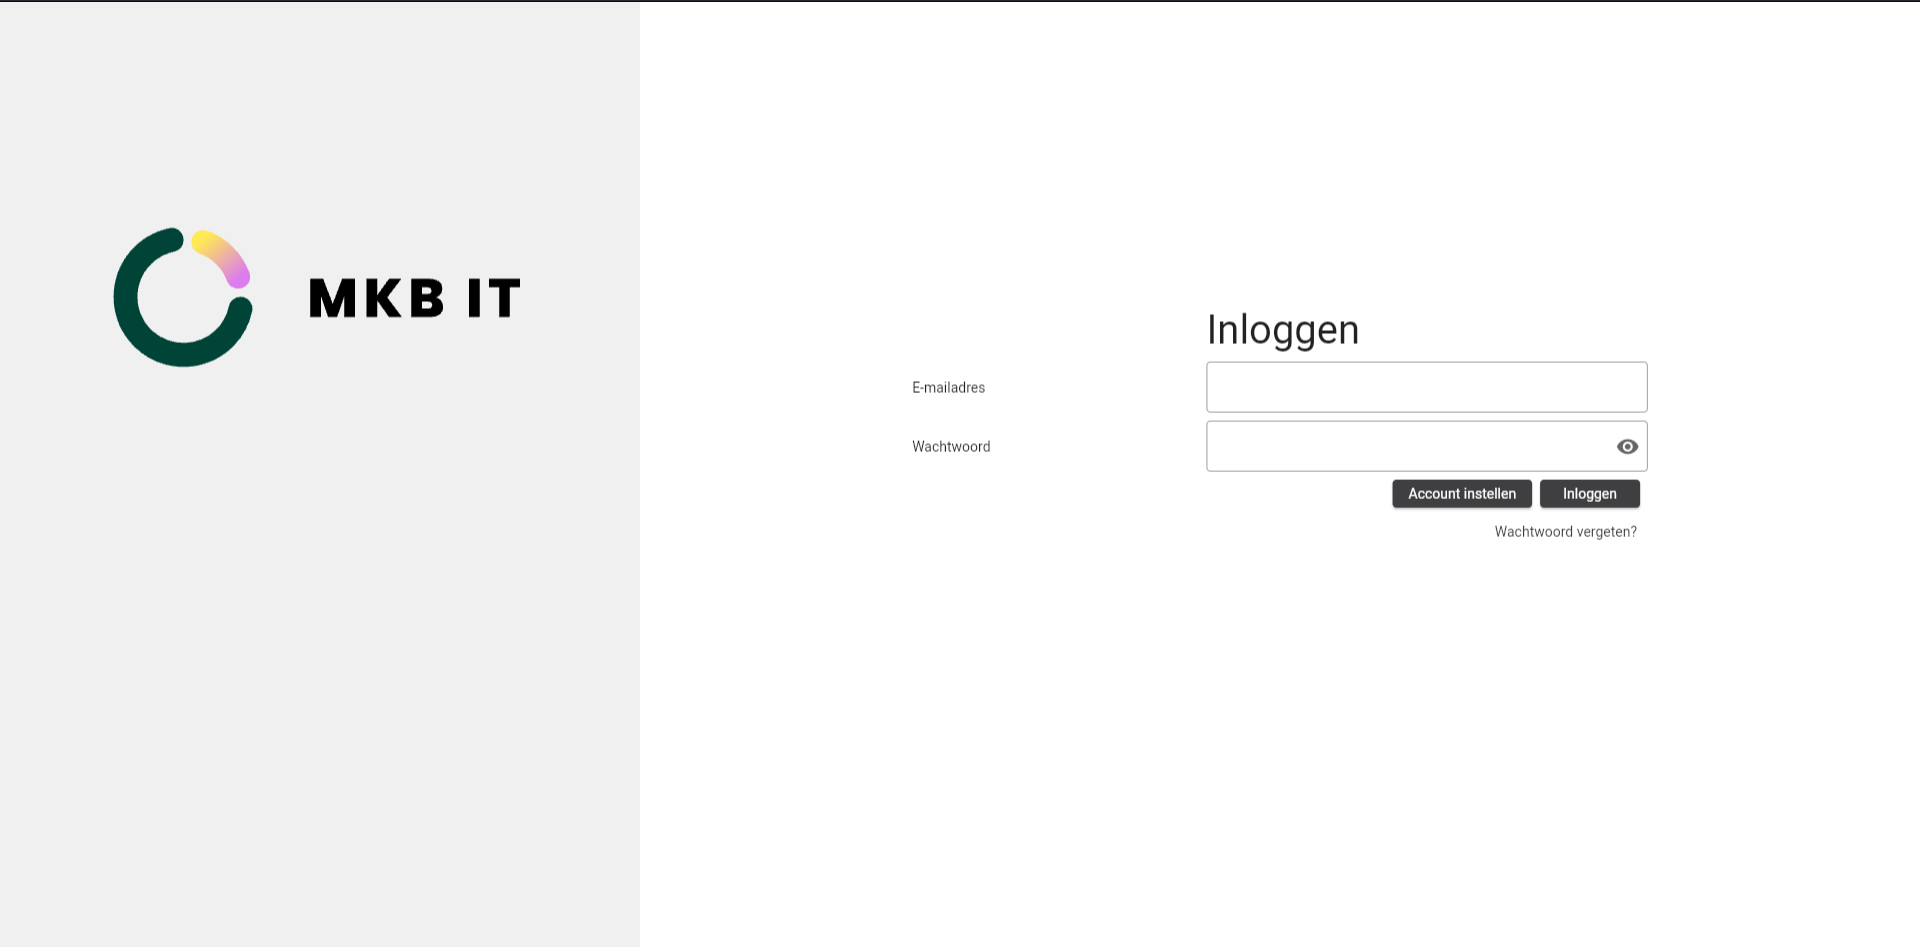
\includegraphics[width=0.8\textwidth]{Figures/Qaas App/Landing Page.png}
      \caption{The login page of the \acrshort{qaas} app, implementing Google \acrshort{2fa} and re\acrshort{captcha}}
\end{figure}

\begin{figure}[htbp]
      \centering
      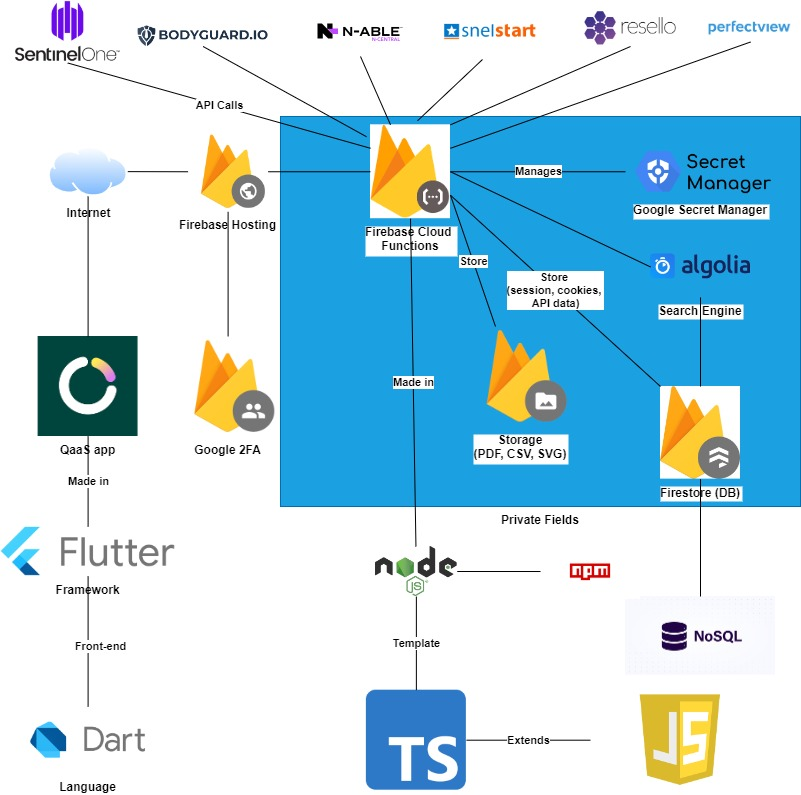
\includegraphics[width=0.8\textwidth]{Figures/QaaS App Infraastructure.jpg}
      \caption{The infrastructure of the QaaS app}
\end{figure}

\begin{multicols}{2}
      \subsubsection{Firebase}
      Firebase is a comprehensive platform for developing and managing web and mobile applications, created by
      Google and is party of \acrshort{gcp}. It was originally an independent company founded by Firebase, Inc.
      in 2011. It was then acquired by Google in 2014. Since then, it has become an integral part of Google's
      broader ecosystem of cloud services (\cite{firebase}). It is a \acrshort{baas} that provides developers with a
      variety of tools and services to help with both back-end infrastructure and front-end capabilities without worrying
      about managing servers or infrastructures. The services offered by Firebase (\textit{\cite{firebaseproducts}}) are
      many, but for this thesis, it will only discuss the ones that are used by the \acrshort{qaas} app. They are listed
      in the following:
      \begin{itemize}
            \item Authentication: is an easy-to-understand authentication services that support various authentication
                  methods like email/password, phone number, with identity providers such as Google, Facebook, Twitter,
                  Apple, GitHub, \acrshort{etc}
                  along with utilizing \acrshort{2fa} authentication factors to enhance security by requiring additional
                  factor, such as an \acrshort{otp} code that is sent to the user's phone or security key.
            \item Database:
                  \begin{itemize}
                        \item Firestore Database: Firestore is a \gls{NoSQL} database that is part of the Firebase
                              platform. It is a flexible, scalable database for mobile, web, and server development. It keeps
                              data in sync across client apps through real-time listeners and offers offline support for mobile
                              and web, so the developers can build responsive apps that work regardless of network latency or
                              Internet connectivity.
                  \end{itemize}
            \item Cloud Functions: often just called Functions in the Firebase console, it allows developers to run
                  back-end code in response to events triggered by Firebase features and \acrshort{https} requests.
                  The code is stored in Google's cloud and runs in a managed environment. It is a serverless framework
                  that allows developers to build and deploy serverless functions that automatically scale up and down
                  based on demand. The available programming languages are Node.js (\acrshort{js} and \acrshort{ts}),
                  Python, Go, Java, and .NET (C\#). Cloud Functions offers 2 product versions: the original version
                  (1st gen), and the 2nd gen which is built on Cloud Run and Eventarc to provide an enhanced feature set.
                  \begin{itemize}
                        \item 1st Generation: Most of the Firebase Cloud Functions that are used in the \acrshort{qaas} app
                              is in this version. The company wishes to migrate all the functions to the 2nd generation in
                              the future. Furthermore, for the integration of SentinelOne with the \acrshort{qaas} app, the
                              company wishes to utilize the 2nd generation of Cloud Functions.
                        \item 2nd Generation: The company wishes that the author's graduation project will utilize the 2nd
                              generation of Cloud Functions. Features in the 2nd generation including:
                              \begin{itemize}
                                    \item Longer request processing times
                                    \item Larger instance sizes
                                    \item Traffic management
                                    \item Eventarc integration
                                    \item Broader CloudEvents support
                              \end{itemize}
                  \end{itemize}
                  Cloud functions are the main back-end infrastructure of the \acrshort{qaas} app. It is used to connect
                  and make \acrshort{http} calls to all the internal \acrshort{api}s. There are different types of
                  functions in Firebase Cloud Functions, and they will be discussed later. Some functions are called within
                  the app, and some outside of the app. Some functions are also used to listen to the Firestore collections,
                  in case of any changes in the data.
      \end{itemize}
\end{multicols}

\begin{figure}[htbp]
      \centering
      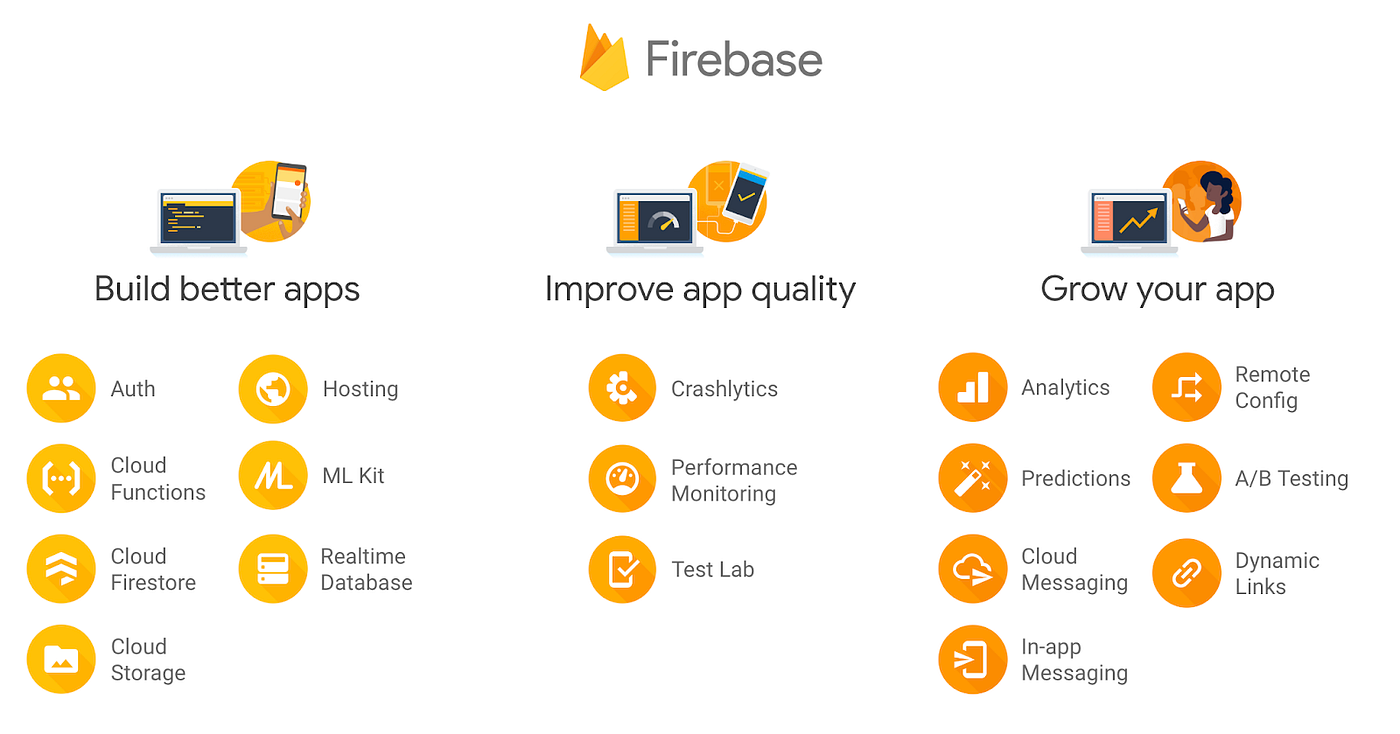
\includegraphics[width=0.8\textwidth]{Figures/Firebase.png}
      \caption{All of the products offered by Firebase (\textit{\cite{firebasePic}})}
\end{figure}

\begin{longtable}{|p{5cm}|p{5.5cm}|p{5.5cm}|}
      \hline
      \rowcolor{blue!20}
      Feature         & 1st Gen                                                     & 2nd Gen                                                       \\
      \endfirsthead
      \hline
      Image registry  & Container Registry or Artifact Registry                     & Artifact Registry only                                        \\
      \hline
      Request timeout & Up to 9 minutes                                             & \begin{itemize}
                                                                                            \item Up to 60 minutes for \acrshort{http}-triggered functions
                                                                                            \item Up to 9 minutes for event-triggered functions
                                                                                      \end{itemize} \\
      \hline
      Instance Size   & Up to 8\acrshort{gb} \acrshort{ram} with 2 v\acrshort{vcpu} & Up to 16\acrshort{gb} \acrshort{ram} with 4 \acrshort{vcpu}   \\
      \hline
      Concurrency     & 1 concurrent request per functions instance                 & Up to 1000 concurrent requests per function instance          \\
      \hline
      \caption{Comparison between the 1st and 2nd Generation of Cloud Functions}
      \label{tab:restvsoap}
\end{longtable}

\begin{figure}[htbp]
      \centering
      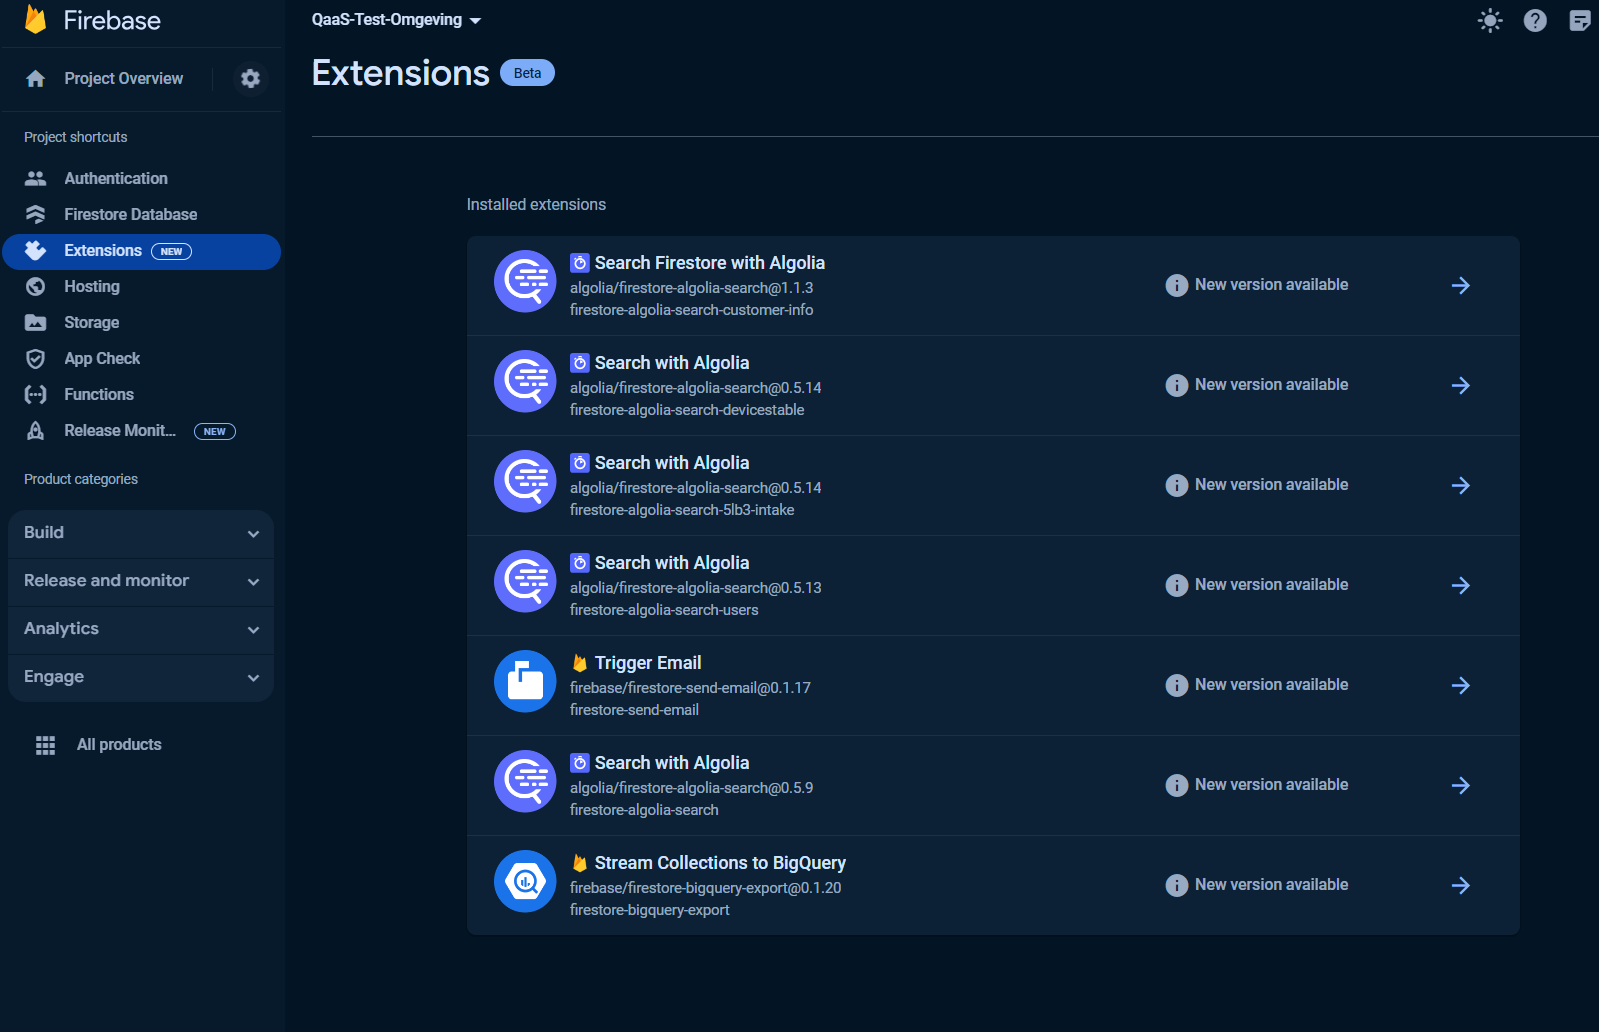
\includegraphics[width=0.8\textwidth]{Figures/Firebase/Extensions.png}
      \caption{All the extensions that are used in the \acrshort{qaas} app, mostly about Algolia}
\end{figure}

\begin{figure}[htbp]
      \centering
      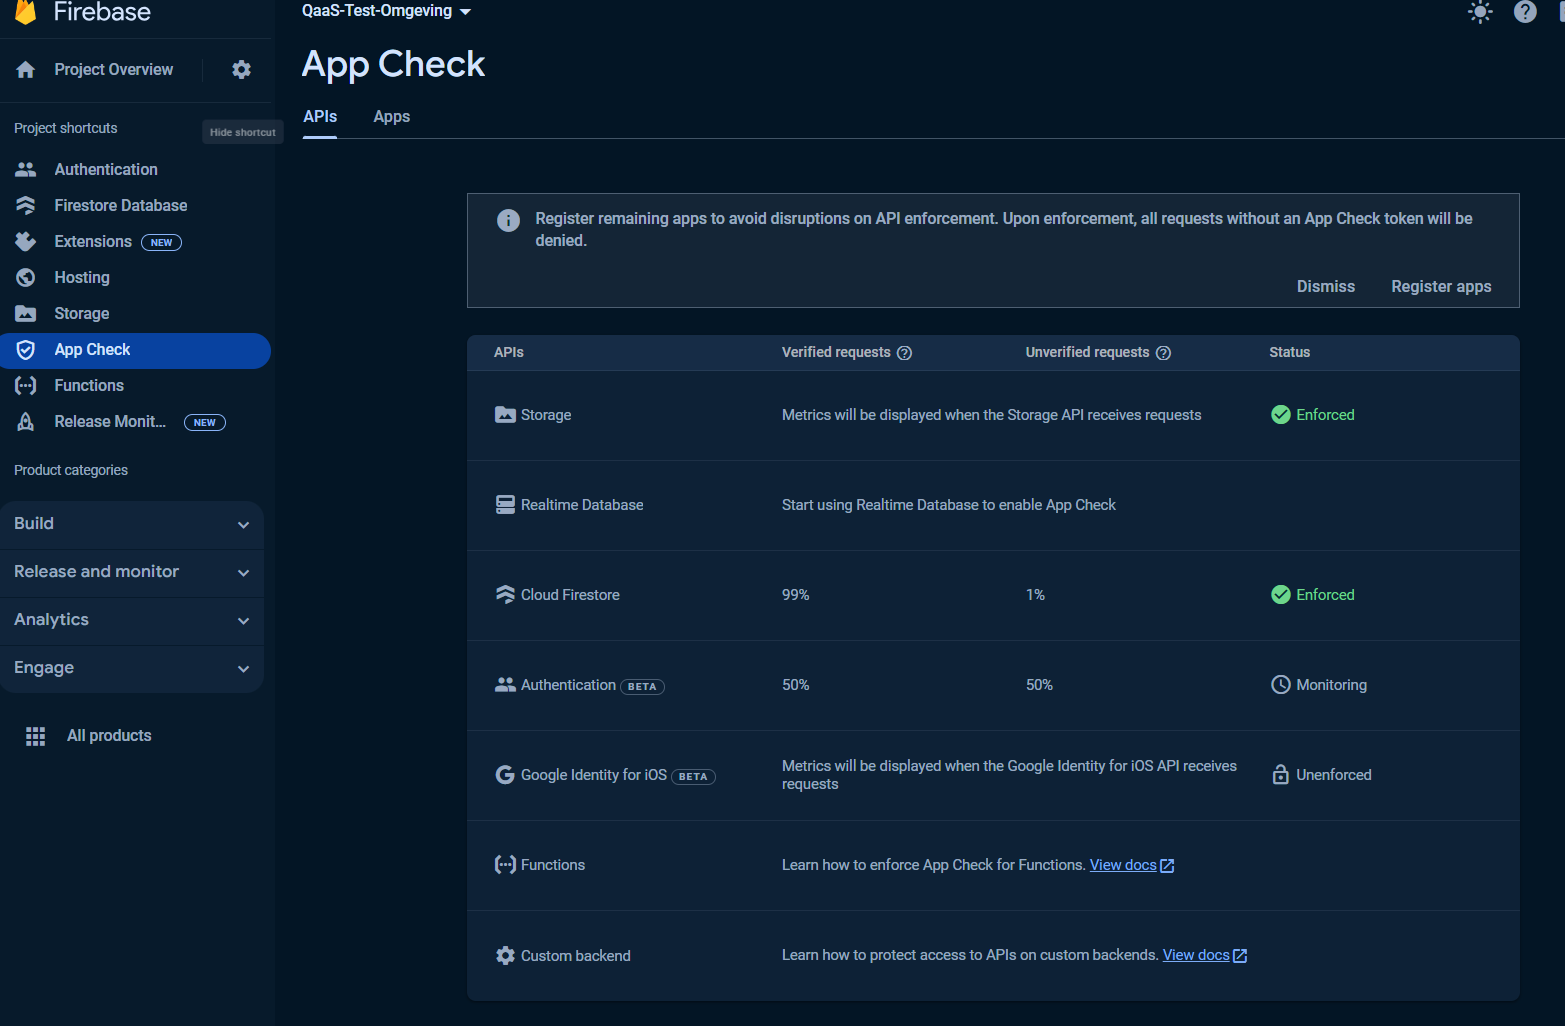
\includegraphics[width=0.8\textwidth]{Figures/Firebase/App Check.png}
      \caption{The App Check feature in the \acrshort{qaas} app}
\end{figure}

\begin{figure}[htbp]
      \centering
      
\includegraphics[width=0.8\textwidth]{Figures/Firebase/Functions/CronJobs.png}
      \caption{The function in the \acrshort{qaas} app that is scheduled to run every 7 days to keep the \acrshort{api} data up-to-date
            (\textit{\cite{cronJobQaaSAppFunction}})}
\end{figure}

\begin{multicols}{2}
      \begin{itemize}
            \item Hosting: a service that allows developers to host static websites, dynamic web apps, mobile apps, and
                  microservices on Firebase's infrastructure. The \acrshort{qaas} app is currently hosted on Firebase
                  Hosting.
            \item Cloud Storage: offers secure, scalable, and reliable file storage and sharing for Firebase apps.
                  It is designed to help developers quickly and easily store and serve user-generated content, such as
                  photos or videos. It is used by the \acrshort{qaas} app to store and serve user-generated content, such as
                  profile pictures, documents, and other files.
            \item Extensions: it consists pre-built, open-source software packages that extend the functionality of a Firebase
                  project (\textit{\cite{firebaseExtension}}). They are designed to automate common development tasks, such as
                  sending notifications, integrating with third-party services, and performing back-end operations, without
                  requiring users to write custom code. The \acrshort{qaas} app uses the Extension mainly for Algolia.
            \item App Check: it is a security feature that, on top of Firebase \acrshort{2fa} Authentication, that helps protect
                  the project from abuse, such as billing fraud or phishing, by ensuring that only the app that is registered
                  can have access to the Firebase project's resources (\textit{\cite{appCheckFirebase}}). In the case of the
                  \acrshort{qaas} app, it uses it \gls{reCAPTCHA} to ensure extra protection in the \acrshort{mfa}.
      \end{itemize}

      \textbf{Different Types of Cloud Functions in Firebase}

      Firebase has a lot of different types of Cloud Functions that developers can use. Just like the previous Firebase product
      explanation, this thesis will only focus on the following types of Cloud Functions that are used in the \acrshort{qaas} app:

      \textbf{HTTP Triggers}: these are functions that are triggered by \acrshort{http} requests. They are used as \acrshort{api}
      endpoints of the \acrshort{qaas} app, allowing server-side logic execution in response to \acrshort{http} requests from
      client-side applications or external services. The requests are GET, POST, PUT, DELETE, and PATCH, and they are used to
      creating, reading, updating, and deleting data in either the Firestore \acrshort{db} or the correlated \acrshort{api}
      environment itself.

      \begin{itemize}
            \item onRequest: this method is used to create an \acrshort{http} function that is triggered by an \acrshort{http}
                  request. They are more general-purpose compared to Callable Functions and can be used to create \acrshort{rest}ful
                  \acrshort{api}s, handle form submissions, or perform any other server-side operations that require \acrshort{http}
                  requests. Unlike Callable Functions, onRequest functions do not handle authentication or data serialization, so
                  the developers need to manage this aspect manually. This functions only accepts \texttt{Request} and
                  \texttt{Response}, but not \texttt{NextFunction}. In the context of \acrshort{qaas} app, this function is only used
                  for testing purposes, and the developer will need to migrate to onCall when deploying on the Live environment.
            \item onCall: is a little different from onRequest. Instead of using Request and Response, it uses data and context.
                  In version 2.0, it only accepts request as \texttt{CallableRequest<any>} that can get any headers and body
                  of the request sent by user. It is used to create Callable Functions, and they are designed to be called directly
                  from client applications, such as mobile or web apps. They automatically handle authentication and data serialization,
                  making it easier to secure call backend code from client applications, and this is what the \acrshort{qaas} app
                  primarily uses for calling its internal \acrshort{api}s as it ensures that the client is authenticated and authorized
                  to make the call. Callable functionsa are triggered by an \acrshort{http} request but are specifically designed to be
                  called from Firebase client \acrshort{sdk}s.

      \end{itemize}
\end{multicols}

\begin{lstlisting}[language=JavaScript, caption=Example of a typical onRequest function]
      import { Request, Response } from 'express';
      import * as functions from "firebase-functions/v2";

      const region = "europe-west1";

      export.getData = functions.https.onRequest({ region: region }, async (request: Request, response: Response): Promise<any> => {
            try {
                  const response = SentinelOneAPICall();
                  return response.status(200).json(data: response.data);
            } catch (ex: unknown) {
                  if (error instanceof Error) {
                        // Error object, log message and stack if available
                        console.error(`[${context}] An error occurred: ${error.message} \n Stack: ${error.stack}`);
                  } else {
                        // Non-Error object, log with a generic message.
                        console.error(`[${context}] An unknown error occurred:`, error);
                  }
                  response.status(500).send("Failed to retrieve agents");
            }
      });
\end{lstlisting}

\begin{lstlisting}[language=JavaScript, caption=Example of onCall function with authentication check]
      import * as functions from "firebase-functions/v2";
      const region = "europe-west1";

      const getData = functions.https.onCall({ region: region }, async (request: CallableRequest<any>) => {
            try {
                  // Checking that the user is authenticated.
                  if (!context.auth) {
                        // Throwing an HttpsError so that the client gets the error details.
                        throw new functions.https.HttpsError('failed-precondition', 'The function must be called while authenticated.');
                  }
                  const response = SentinelOneAPICall();
                  return {
                        data: response.data,
                  };
            } catch (ex: unknown) {
                  if (error instanceof Error) {
                        // Error object, log message and stack if available
                        console.error(`[${context}] An error occurred: ${error.message} \n Stack: ${error.stack}`);
                  } else {
                        // Non-Error object, log with a generic message.
                        console.error(`[${context}] An unknown error occurred:`, error);
                  }
                  throw new functions.https.HttpsError("unknown", "Failed to retrieve agents", ex);
            }
      });

      async function SentinelOneAPICall() : Promise<any> {
            const apiUrl = 'https://sentinelOne.example.com/users/123';

            // Define the request parameters
            const requestOptions = {
                  method: 'GET', // HTTP method (GET, POST, PUT, DELETE, PATCH, etc.)
                  headers: {
                        'Content-Type': 'application/json', // Set the content type of the request
                  }
            };
      
            // Make the API request
            fetch(apiUrl, requestOptions)
                  .then(response => response.json())
                  .then(data => console.log(data)) // Process the response data
                  .catch(error => console.log('error', error)); // Handle any errors that occurred during the request
      }
              
      export = getData;
\end{lstlisting}

\begin{multicols}{2}
      \textbf{Pub/Sub Triggers}: are the functions triggered by messages published to a \acrshort{pubsub} topic.
      It is a messaging service that enables decoupling of applications by sending messages between independent components.

      \textbf{Cloud Firestore Functions}

      \textbf{Schedule functions}: this is a Firebase's own term for \gls{cronJob} (\textit{\cite{scheduleFunction}}).
      They are used within the \acrshort{qaas} app to run tasks at regular intervals, such as sending reminders, keeping
      data up-to-date with the internal \acrshort{api}s (like customer list), or performing maintenance tasks.

      \textbf{Algolia}

      Algolia is used for search functionality. It is a search-as-a-service platform that enables developers to
      integrate and build fast, relevant search functionality into their applications and websites
      (\textit{\cite{algolia}}). It provides a range of features and capabilities for building and managing search
      functionality, including full-text search, typo tolerance, and relevance tuning, as well as analytics and
      monitoring tools to help developers understand how users are interacting with their search functionality in
      real-time.

      The reason as to why \acrshort{qict} uses Algolia is that the nature of Firebase search engine is quite often
      proven to be inaccurate and slow.

      \textbf{Google Secret Manager}

      It is a fully managed service provided by \acrshort{gcp} that allows developers and organization to securely store,
      access, and manage sensitive information such as API keys, passwords, certificates, \acrshort{oauth} credentials,
      \acrshort{db} credentials and other credentials used in throughout the lifecycle of their applications
      (\textit{\cite{googlesecretmanager}}). It is not part of Firebase, and it helps the \acrshort{qaas} app to centralize and
      secure its secrets in scalable and easily manageable way. Key-features of Secret Manager include:

      \begin{itemize}
            \item Secure Storage: it encrypts the secret values using \acrshort{cmek}, ensuring the sensitive data is protected
                  both at rest and in transit.
            \item Audit Logs: it provides and manages audit logs that record all access and modification of activities, helping
                  developers meet compliance, better accountability and regulatory requirements.
            \item Versioning and Automatic Rotation: it supports versioning of secrets, allowing developers to store multiple versions
                  of the same secret. This means that the developers get to keep multiple versions of secrets and easily revert or roll
                  back to a previous version if needed, which will help in auditing and tracking changes to secrets over time. This feature
                  enables automatic seamless rotation of secrets at regular intervals without  disrupting the applications, which improves
                  the security part of the application by ensuring that secrets are regularly updated without manual intervention.
            \item Access Control: it provides fine-grained access control using Google \acrshort{iam}, allowing developers to specify
                  who can access and manage the stored secrets and what they can do with them.
            \item Centralized Management: it stores and manages all secrets in one place, simplifying access and control.
      \end{itemize}

      Google Secret Manager comes from \acrshort{gcp}, and \acrshort{gcp} and Firebase are a separate cloud solutions. But, because
      both are part of Google, Firebase Cloud Functions can typically access \acrshort{gcp} Secret Manager by editing that specific function
      that the developer wanted to grant access to.

      \subsubsection{Modules and Templates of the QaaS App}

      The \acrshort{qaas} has several templates and modules that are used to build the app. The templates can be
      interpreted as level of access to the app, showing what permission a user has to the app. There are 3 different
      templates based on 3 different users:

      \begin{itemize}
            \item \textbf{Clients}: this template is used by the general users of the app. They have limited access to
                  the app's features and functionalities, such as viewing and updating their profile and accessing the app's
                  resources. They can only see the data relevant to their own account and cannot access or modify data
                  belonging to other client from different company.  The Client template is designed for users who have the
                  lowest level of access and control over the app.
            \item \textbf{Helpdesk}: this template is used within the Helpdesk department of \acrshort{qict}. They have more
                  access to the viewing of app functionality than the Clients.
            \item \textbf{IT Admin}: the \acrshort{it} admin have almost the same level of access as the Helpdesk. The only
                  difference is that they have the ability to create, edit, and delete users, manage user permissions, and
                  configure the app settings. They can also grant and revoke access to a user and to the app's features and
                  functionalities, which are called Modules. The admin template is designed for users who have the highest level
                  of access and control over the app, which is to the developers.
      \end{itemize}

      Modules are

      User tags are used for differentiating different companies.
\end{multicols}

\begin{figure}[htbp]
      \centering
      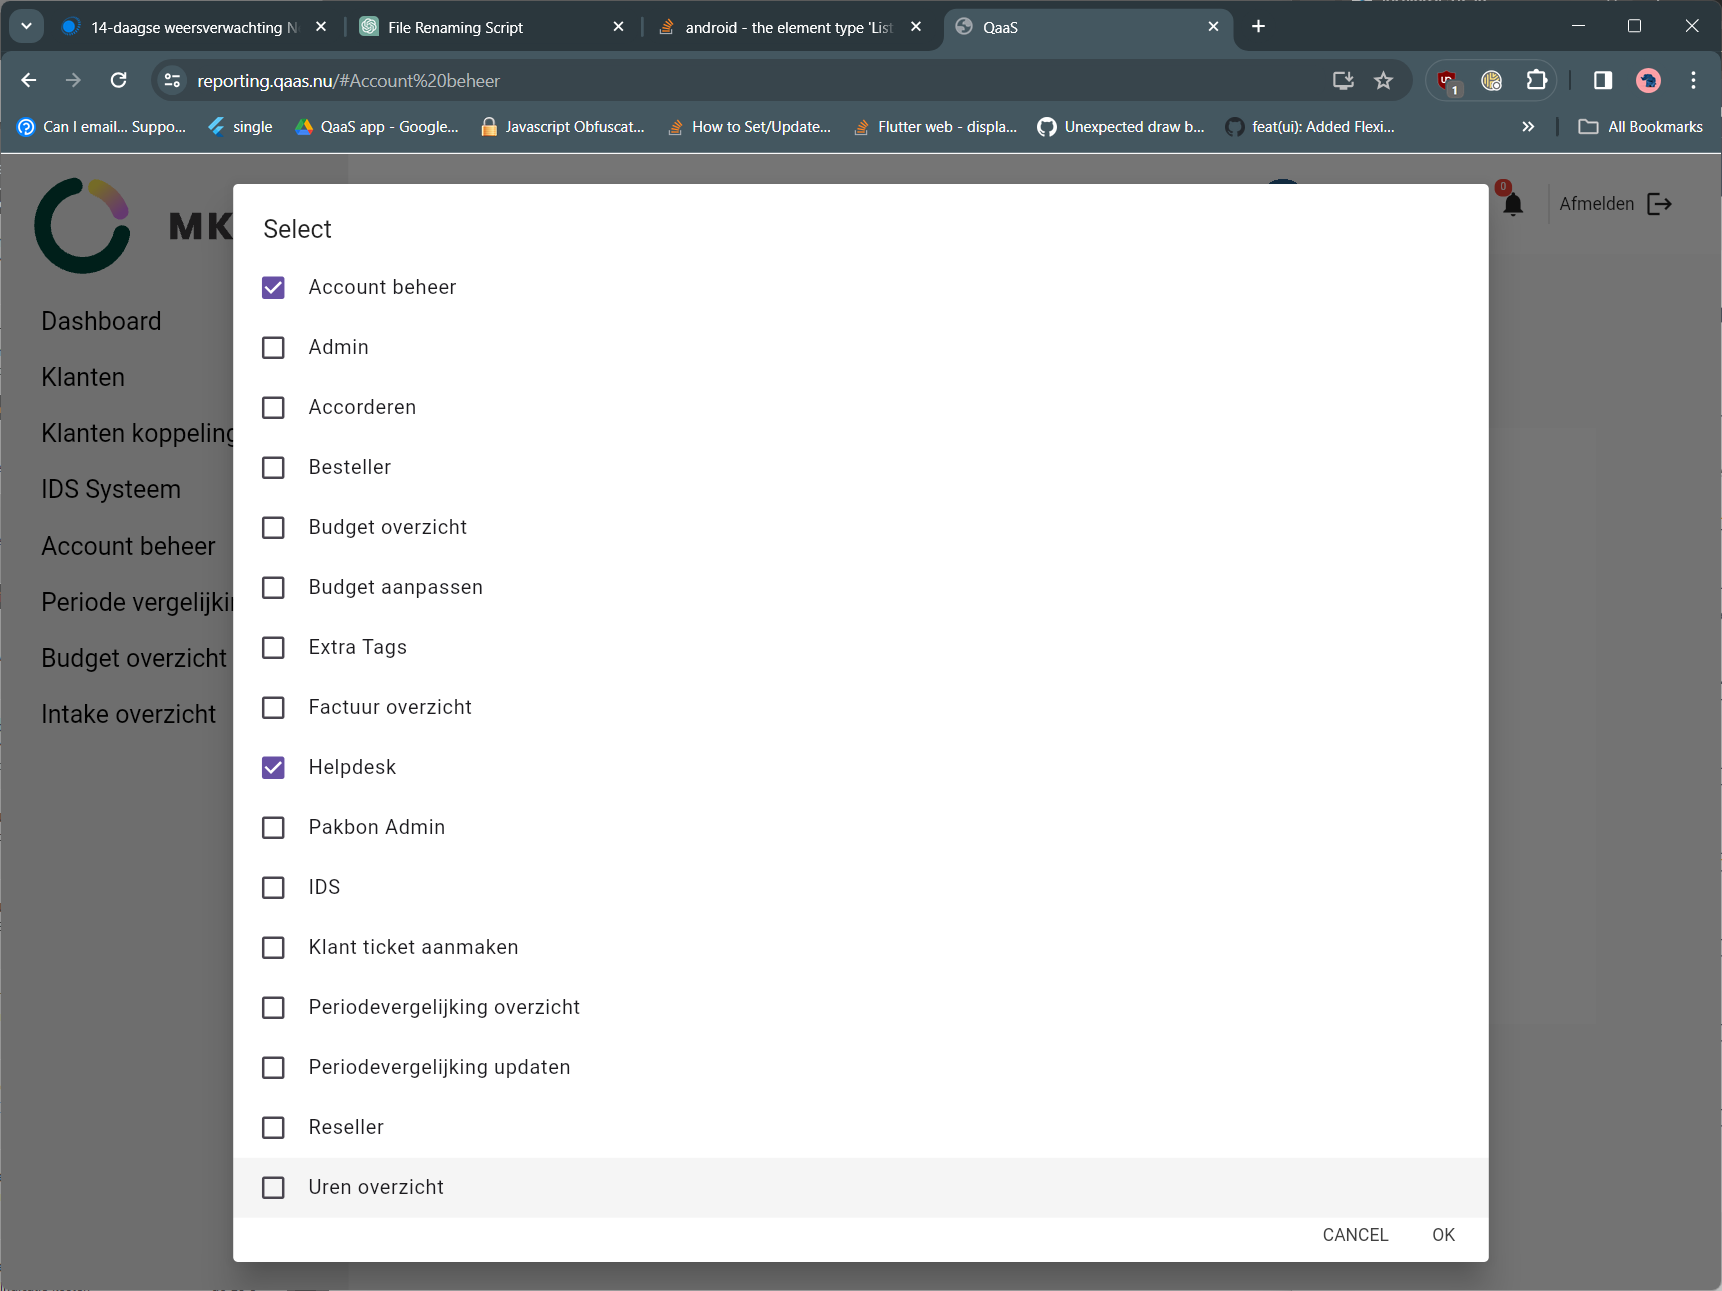
\includegraphics[width=0.8\textwidth]{Figures/Qaas App/Modules/afbeelding (1).png}
      \caption{Different modules in the QaaS app in which the IT admin can determine which pages can be accessed by which user tags}
      \label{fig:qaasAppModules}
\end{figure}

\begin{figure}[htbp]
      \centering
      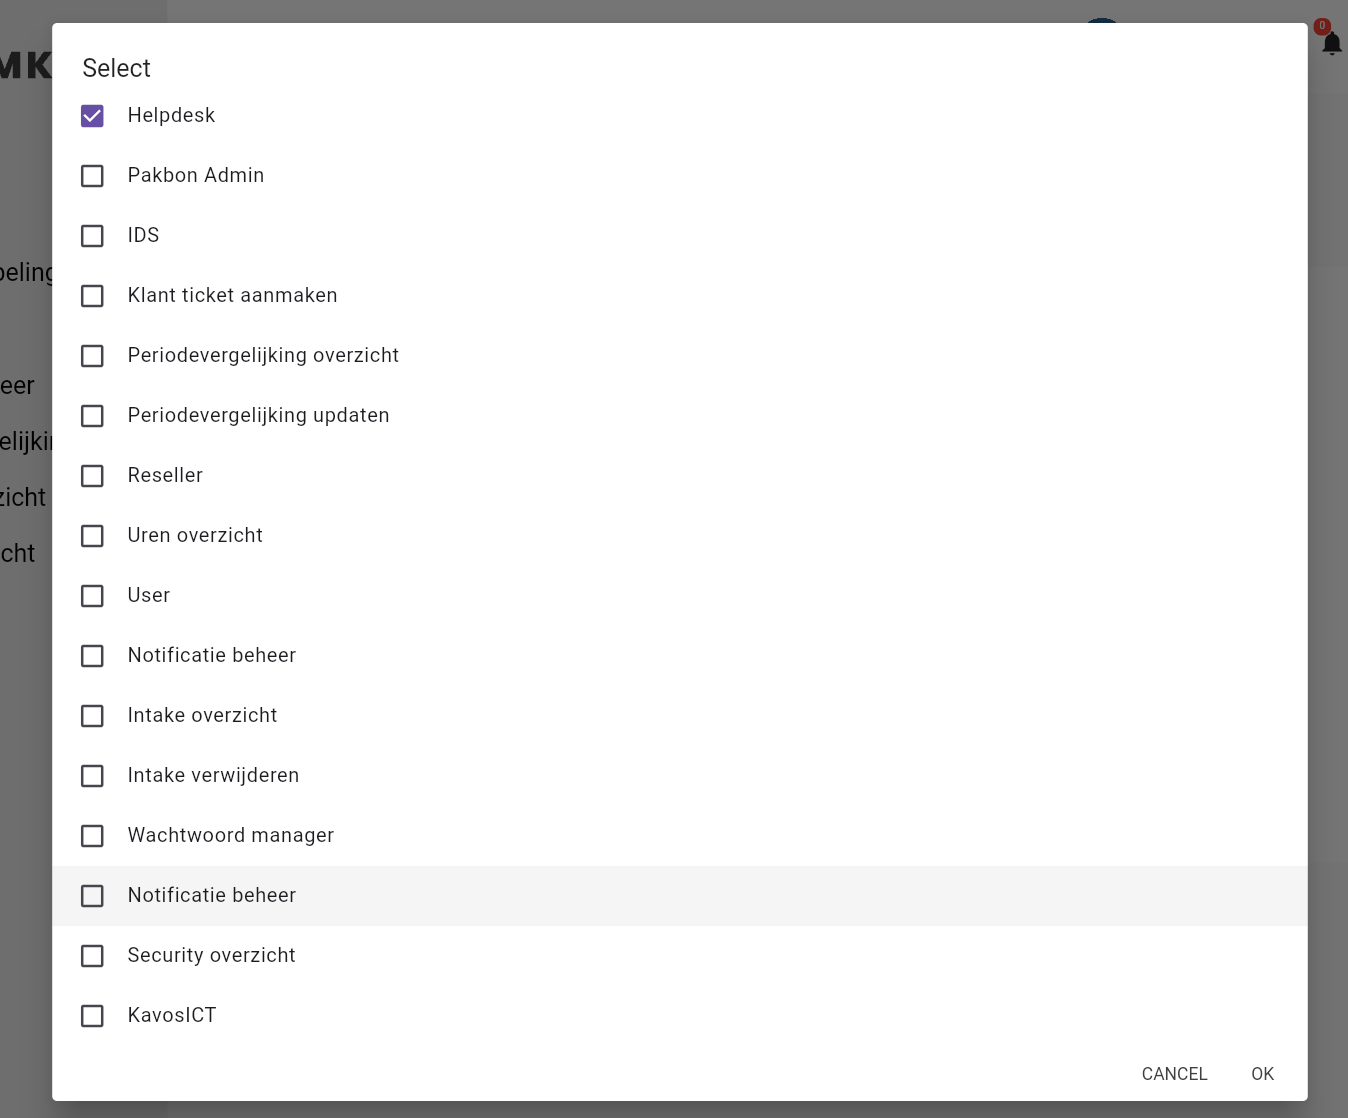
\includegraphics[width=0.8\textwidth]{Figures/Qaas App/Modules/afbeelding (2).png}
      \caption{Different user tags in the QaaS app in which correlates to what actions can a user do within the web application}
      \label{fig:userTages}
\end{figure}

\begin{multicols}{2}
      \subsection{Conclusion}
      The \acrshort{qaas} app is an \acrshort{erp} web application that is used by \acrshort{qict} and its clients.
      It is made in Dart with Flutter as the front-end framework, and Node.js with the back-end  framework with
      TypeScript as a template to ensure type safety. The back-end is hosted on Firebase Cloud Functions, and the
      front-end is hosted on Firebase Hosting. The app uses several internal \acrshort{api}s and technologies to
      help with its operations, such as Resello, SnelStart, Bodyguard.io, N-Central, and PerfectView. The app also
      uses several Firebase products, such as Authentication, Firestore Database, Cloud Functions, Hosting, Cloud
      Storage, Extensions, App Check, and Google Secret Manager. The app also uses Algolia for search functionality. The app
      has several templates and modules that are used for the authentication and authorization of the app.
      The templates control what 3 different types of users can do in the app, they are Clients, Helpdesk, and IT
      Admin. The modules help with the control of the app's features and functionalities, and the IT Admin has the
      highest level of access and control over the app.

      \section{Research Sub-Question \#2: What is SentinelOne EDR Platform?}
      % vs CrowdStrike with Carbanak and FIN7 methodology, Huntresss, datto rmm

      SentinelOne is a cybersecurity platform that provides endpoint protection, detection, and response capabilities to
      help organizations defend against advanced cyber threats. It leverages \acrlong{ai} and machine learning to analyze
      and respond to security threats in real-time, providing organizations with comprehensive protection against malware,
      ransomware, and other cyber threats. It also provides visibility into clients' \acrshort{it} systems and infrastructure,
      enabling organizations to gain insights into potential security risks and vulnerabilities and take proactive measures
      to address them.

      Some terminology that the readers need to be familiar with before diving deeper into SentinelOne:

      \textbf{Endpoint}

      Endpoint can be defined as any remote computing devices that receives incoming communications and sends outgoing messages
      to the network it is connected to. Examples of endpoints include desktops, laptops, smartphones, tablets, servers, workstations,
      and other \acrshort{iot} devices that is connected to a network. They are the first-line of defence for the Blue Team today.

      Examples of endpoints are:
      \begin{itemize}
            \item Computer (workstations, desktops)
            \item Laptop
            \item Server
            \item Mobile devices
      \end{itemize}

      \textbf{EPP}

      \acrshort{epp} is an upgrade from legacy \acrshort{av}/anti-malware. \acrshort{epp} consists of solutions that work together to detect
      and block security threats at the endpoint device level.

      Important note that \acrshort{epp} is not to be confused with \acrshort{edr}. \acrshort{epp} is a separate service from \acrshort{edr},
      in which in \acrshort{edr} platforms they often include \acrshort{epp} but not vice versa.

      \textbf{EDR}

      \acrshort{edr} \acrshort{aka} \acrshort{etdr}, is a group of integrated endpoint security solutions that combine data collection,
      data analysis, forensics, and \gls{threathunting} with the end-goal of identifying and stopping any potential security breaches in due
      time. \acrshort{edr} solutions are able to recognize any suspicious patterns that can be investigated later on, as they have been
      purposefully created to detect and respond in an active manner to advance malware, ransomware, and other cyber threats (the Response
      \acrshort{edr}). \acrshort{edr}, as the name suggest, were developed specifically for endpoints, and not networks (\ref{sec:ndr}), thus
      operate only on endpoint level.

      The number one thing that sets apart \acrshort{edr} from legacy (traditional) \acrshort{av} is that traditional \acrshort{av} relies on
      signature-based detection, usually having a defined set of list in their \acrshort{db}, where known malware signatures are compared
      against files or processes to identify threats. \acrshort{edr} on the other hand, uses a combination of signature-based detection, such
      as behavioural analysis, machine learning, and anomaly detection to identify and respond both known and unknown threats. \acrshort{edr}
      solutions focus on detecting malicious activities at the endpoint level, including file modifications, process execution, and network
      connections, focusing on malicious behaviour compared to only concerning with malicious software like what traditional \acrshort{av} does.

      \textbf{MDR}

      \acrshort{mdr} is what manage the \acrshort{edr} technology.

      \textbf{NDR} \label{sec:ndr}
      \acrshort{ndr} products are designed to provide a complete visibility into the network, real-time detection of threats, and guided
      investigation to accelerate and automate responses (\textit{\cite{sentinelOneNDR}}). \acrshort{ndr} takes a feed of raw network traffic
      from a \gls{networkTap}, port mirror, or virtual traffic mirroring in \acrshort{aws} and Azure. By analyzing this traffic in real-time,
      \acrshort{ndr} finally discovers and classify every device communicating on the network. It identifies device roles, such as \acrshort{dns},
      web server, medical device, \acrshort{etc} and maps peer groups among those devices.

      \textbf{SIEM}

      is a software system that collects, aggregates, normalizes security data from a variety of sources within an IT infrastructure, and
      analyzes it according to pre-set rules, present it in human-readable format and therefore giving a comprehensive picture of the company's
      information security (\cite{siemGartner}). \acrshort{siem} tools evolved from the log management discipline and combine \acrshort{sim} and
      \acrshort{sem} technologies. A \acrshort{siem} tool uses \acrshort{ai} to automate several manual procedures related to threat
      detection and incident response. Furthermore, it assists enterprise security teams in spotting anomalies in user behavior.

      \begin{itemize}
            \item Input: logs, threat intel, vulnerability feeds, \acrshort{ndr}, firewall, \acrshort{ips}, \acrshort{ids}, and \acrshort{edr}
                  data
            \item Output: high-fidelity alerts prioritized by severity
            \item Infused with: \acrshort{ai}, \acrshort{ml}, and analytics
      \end{itemize}

      \textbf{SOAR}

      \acrshort{soar} solutions focus on automating incident response processes and triage capabilities. The key word here is
      "orchestration" and "automation". In an ideal world, everything.
      The main goal is to oversee security without human help as much as possible, boosting productivity and shortening the response time.
      It might use \acrshort{ai} and \acrshort{ml} to assess security events and automate incident response procedures. These solutions
      can be standalone product, or it can be added to \acrshort{siem} solutions since \acrshort{soar} does not excel in event analysis.

      \textbf{XDR}

      is a security solution that gathers and analyzes data from multiple sources like endpoints, networks, cloud, emails, app,
      \acrshort{etc} It offers great visibility into a company's \acrshort{it} infrastructure, helping the security employees to detect
      more threats, respond efficiently, and deal with fewer false positive alerts \cite{xdrIDC}.

      This solution integrates several tools combining all the gathered data into a single platform to visualize the information. It might
      incorporate automated processes (even complex ones), \acrshort{ml}, and advanced analytics to enable quicker and more effective
      incident response. It can even deal with hidden and advanced malware.

      \textbf{MXDR}

      Some people may still call it \acrshort{mdr}, managed \acrshort{soc}, or managed security.

      \textbf{SOC}

      \acrshort{soc} is the organizational context itself. It is a centralized facility or team within an organization that houses a
      security team responsible for monitoring and analyzing another organization's (client) security position on an ongoing basis. They
      can be seen as the safety team for client organizations. Please note that SentinelOne company itself is not a \acrshort{soc}, as it
      is just a cybersecurity company that offers endpoint security solutions.

\end{multicols}

\begin{figure}[htbp]
      \centering
      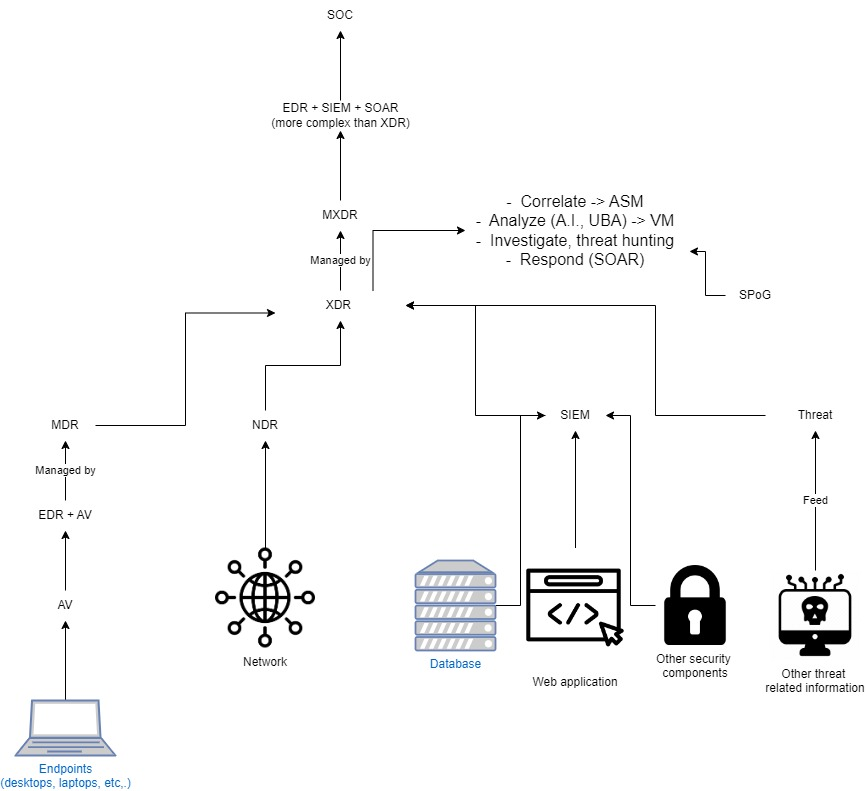
\includegraphics[width=0.8\textwidth]{Figures/XDR.jpg}
      \caption{How all terms related to various technologies in cybersecurity connected to each other}
      \label{fig:xdr}
\end{figure}

\begin{multicols}{2}
      \textit{Please note that as mentioned before, \acrshort{siem} can also take data from an \acrshort{edr} and \acrshort{ndr} but for
            the sake of simplicity, the diagram puts them as a separate pier systems}. In terms of SentinelOne, it has all the features that
      are mentioned in the diagram, except for \acrshort{soc}, as was mentioned before.

      \textbf{Console}

      \textbf{Global}

      The Global tab refers to the environment of the highest level of advisors. It consists of organizations that have access to global level
      that propagate down to the tenant level, which means they can put policies, scripts, and other configurations that will be applied to all
      console and all of their customers.

      \textbf{Tenant}

      \textbf{Mentees}

      \textbf{Site}

      Site is just a name

      \textbf{Group}

      Group refers to logical grouping of devices within SentinelOne \acrshort{mgmt} Console. Groups can be created and deleted by the
      admin user, and

      \textbf{Agents}

      An Agent is a software program, part of SentinelOne product, that is deployed to each endpoint, including desktop, laptop,
      server or virtual environment, and runs autonomously on each device, without reliance on Internet connection, enabling data
      gathering, detection, and response to actions. Agents can be interpreted as an \acrshort{av}, collecting relevant security
      telemetry such as:
      \begin{itemize}
            \item Running processes
            \item Connected servers
            \item Open files
      \end{itemize}
      This information can be useful to detect the presence of a threat or to use in forensic analysis and investigation after
      an attack has occurred (Recovery).

      \textbf{Ranger}

      Ranger is an add-on SentinelOne product that provides a way of detecting other devices (computers and
      \acrshort{iot} devices) that are on the client's computer network. If a malicious attacker comes in and plugs his device
      into the network, all the other SentinelOne agents are going to read the network traffic, determine and classify whether
      that is a new device or a rogue device. As long as a device has Ranger on that network subnet, SentinelOne can gather and
      detect technical information regarding the device.

      \begin{itemize}
            \item Not reviewed
            \item Not trusted
            \item Under analysis
            \item Allowed
      \end{itemize}

      Ranger is designed to detect and take out malicious actors that are in the local subnet, as they can a lot of information about the
      devices (\textit{see \acrshort{arp} Poisoning \cite{arpSpoofing} and man-in-the-middle-attack \cite{man-in-the-middleAttack}}).
      In the real-business scenario, a lot of the times, a company has a very secure perimeter firewall
      (\textit{the big outer castle wall in castle-and-moat network security model \cite{castleMoatWallNetwork}}), but the inside network
      are wide open (unless they are doing logical separations of their local network, such as using \acrshort{vlan}) for attacks inside
      the network.

      Unfortunately for this project scope, Ranger \acrshort{api} calls are off limit, as the company is still..., therefore displaying all
      the Ranger ability to scan and the \acrshort{api} call of the author's account.

      \textbf{Sentinels}

      Sentinels refer to a term that describes SentinelOne ability to deploy and manage security agents on endpoints within an
      organization, not part of SentinelOne product, like Ranger. This is part of the SentinelOne \acrshort{edr} capabilities,
      where the user admin can deploy the agents on the endpoints, and manage them from the SentinelOne console. The admin can
      also create policies, scripts, and other configurations that will be applied to all the agents in the network.

      \textbf{Visibility}

      Unfortunately, \acrshort{qict} does not have Visibility turned on its tenant, thus this feature is also off limit for this project
      scope. But in general, Visibility allows users to do deep querying to be able to identify different things, such as attributes of
      a machine. It is useful when user is looking for threats or any additional information in Incident Response or \gls{threathunting},
      which in most cases is proactive, Visibility can give the user a lot of power to use queries, and interrogate all the information
      or telemetry that SentinelOne has pulled off from the connected machines.

      \textbf{Incidents}

      Incident is just a name of a page in SentinelOne dashboard that provides a list of cyber-incidents overview that have happened on all
      endpoints detected by Agents in the network connected to SentinelOne by Ranger. The page typically offers an overview of all detected
      security incidents, categorized based on severity levels of types of threats.

      Once a threat is detected, the user can take the following actions in the dashboard, if they have enough privileges
      to do so:
      \begin{itemize}
            \item Kill: stops all processes related to that threat
            \item Quarantine: encrypts and moves the threat and its executables
            \item Remediate: deletes all files and system changes created by the threat
            \item Rollback: restores files and configuration that the threat changed. This step is usually taken when a malware has
                  executed its script and has made changes to the system, \acrshort{eg} a ransomware has encrypted all the files and
                  asked for a ransom. By taking this step, all the three previous steps will also be undertaken as well. This will
                  then reboot the system and restore it to the safe state before the malware has been executed.
      \end{itemize}

      \textbf{Reports}

      The reports in SentinelOne provide users with insights into the security posture and threat landscape across their organization's
      endpoints. The reports offer customizable reporting capabilities, allowing users to generate reports tailored to their specific
      requirements. Users can then choose from a variety of predefined report templates or create custom reports based on their unique
      needs.

      Furthermore, the users can also choose for the report to be made automatically, instead of manually filling them themselves. They can
      schedule automated report generation at regular intervals, such as daily, weekly, or monthly.
\end{multicols}

\begin{figure}[htbp]
      \centering
      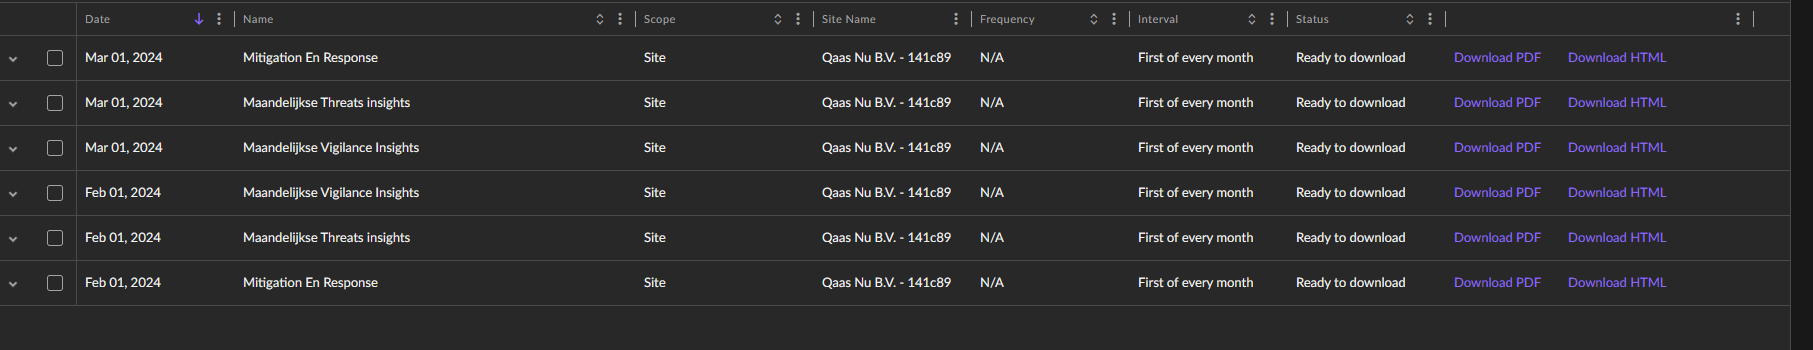
\includegraphics[width=1.0\textwidth]{Figures/SentinelOne/Reports.png}
      \caption{Examples of automatic reports that can be downloaded in SentinelOne}
      \label{fig:Reports}
\end{figure}

\begin{multicols}{2}
      \textbf{Vigilance}

      It is a \acrshort{mdr} service - providing threat monitoring, hunting, and response, to its existing customers. It
      provides a 24/7 \acrshort{soc} with expert analysts and researchers to give customers near real-time threat monitoring,
      in-console threat annotations, and response to threats and suspicious events. Vigilance itself is a separate package from
      SentinelOne.

      \textbf{\textit{How does SentinelOne get all this information from a device without having them even connected to the Internet?}}

      On a network, before a machine is connected and talks to other devices
      and gateways, it is going to do a broadcast and gives up information about itself. This is called an \acrshort{arp} Request.
      As everything that is talking on Layer 2 is giving out their \acrshort{mac} address for exchange,

      A lot of the times, most switches and routers do not change their default credentials

      As was said before, every single item that is connected to a network is constantly broadcasting information out to the rest of
      network, in order to get and maintain an \acrshort{ip} address to keep accessing the Internet, even when it is not actively using
      it (\textit{see \acrshort{dhcp} Protocol \cite{dhcpProcess}}). In case of an endpoint that has SentinelOne installed on it that
      has Ranger, that Ranger is going to listen to that \acrshort{nic} on that device, then capture and interpret all the data that
      is flowing across the network, called \acrshort{mib}s, thus displaying it on the Console.

      \section{Research Sub-Question \#3: How can SentinelOne be integrated with the QaaS app?}

      SentinelOne provides an \acrshort{api} to allow users to integrate SentinelOne with other security tools and systems. Additionally,
      SentinelOne also provide an \acrshort{sdk} enables organizations to scan files and detect malicious content among them, called
      Nexus Embedded \acrshort{ai} (\textit{\cite{nexusSDK}}), but this thesis will focus solely on SentinelOne \acrshort{api}s.

      SentinelOne also provides a comprehensive documentation for its \acrshort{rest}ful \acrshort{api} that allows users to interact
      with the SentinelOne platform programmatically. The \acrshort{api} provides a wide range of functionalities, including the ability
      to retrieve information about devices, incidents, and threats, as well as the ability to perform actions such as quarantining devices,
      remediating threats, and generating reports. The \acrshort{api} is designed to work with the Agents, Sentinels, Ranger, and other
      components of the SentinelOne platform.

      The \acrshort{api} sends requests to the associated Management Server and responds with the data that the management pulled from
      the Agents or from the management database. Therefore, all the data that is displayed in the SentinelOne Console dashboard is also
      available through the \acrshort{api}.

      \textbf{API Token}

      To be able to access SentinelOne \acrshort{api}s, the user needs to have an \acrshort{api} token to prove their
      identity and that their organization has SentinelOne subscription, therefore has right to access data.
      \acrshort{api} tokens can be created in the SentinelOne \acrshort{mgmt} Console.

      The \acrshort{api} token will be shown only once; therefore the user needs to store it in a secure place.
      The token generated by the user is time-limited. To renew the token, the user must generate a new one with
      the same above-steps.

      \subsection{Conclusion}
      SentinelOne is a cybersecurity platform that provides endpoint protection, detection, and response capabilities
      to help organizations defend against advanced cyber threats. It leverages \acrshort{ai} and machine learning to
      analyze and respond to security threats in real-time, providing organizations with comprehensive protection against
      malware, ransomware, and other cyber threats. % SentinelOne provides a wide range of features and capabilities, including
      % endpoint protection, detection, and response, as well as visibility into clients' \acrshort{it} systems and infrastructure.
      SentinelOne also provides a \acrshort{rest}ful \acrshort{api} that allows users to interact with the SentinelOne platform
      programmatically, enabling integration with other security tools and systems. The \acrshort{api} provides a wide range of
      functionalities, including the ability to retrieve information about devices, incidents, and threats, as well as the ability
      to perform actions such as quarantining devices, remediating threats, and generating reports. The author will use the official
      SentinelOne \acrshort{api} documentation to integrate SentinelOne with the \acrshort{qaas} app to display the data of
      \acrshort{qict} and its 400 clients in the \acrshort{qaas} app. The functionality such as filtering, sorting, and pagination
      will also be taken into account to make the data more user-friendly. The author will utilize different kinds of Firebase Cloud
      Functions (\acrshort{http} onCall, Pub/Sub Triggers, Schedule functions) to call the SentinelOne \acrshort{api}s and display
      data. Firestore will also be used to store the user's preference from the \acrshort{qaas} app, such as the user's choice of
      what data they want to see, and visualization types. The author will also utilize Google Secret Manager to store the
      \acrshort{api} token and other sensitive information securely, so it will not be displayed in the code to avoid any security
      risks. Furthermore, \acrshort{ai} powered search engine Algolia will be used to search for specific data in the \acrshort{qaas} app,
      as well as Firestore

\end{multicols}

\begin{figure}[htbp]
      \centering
      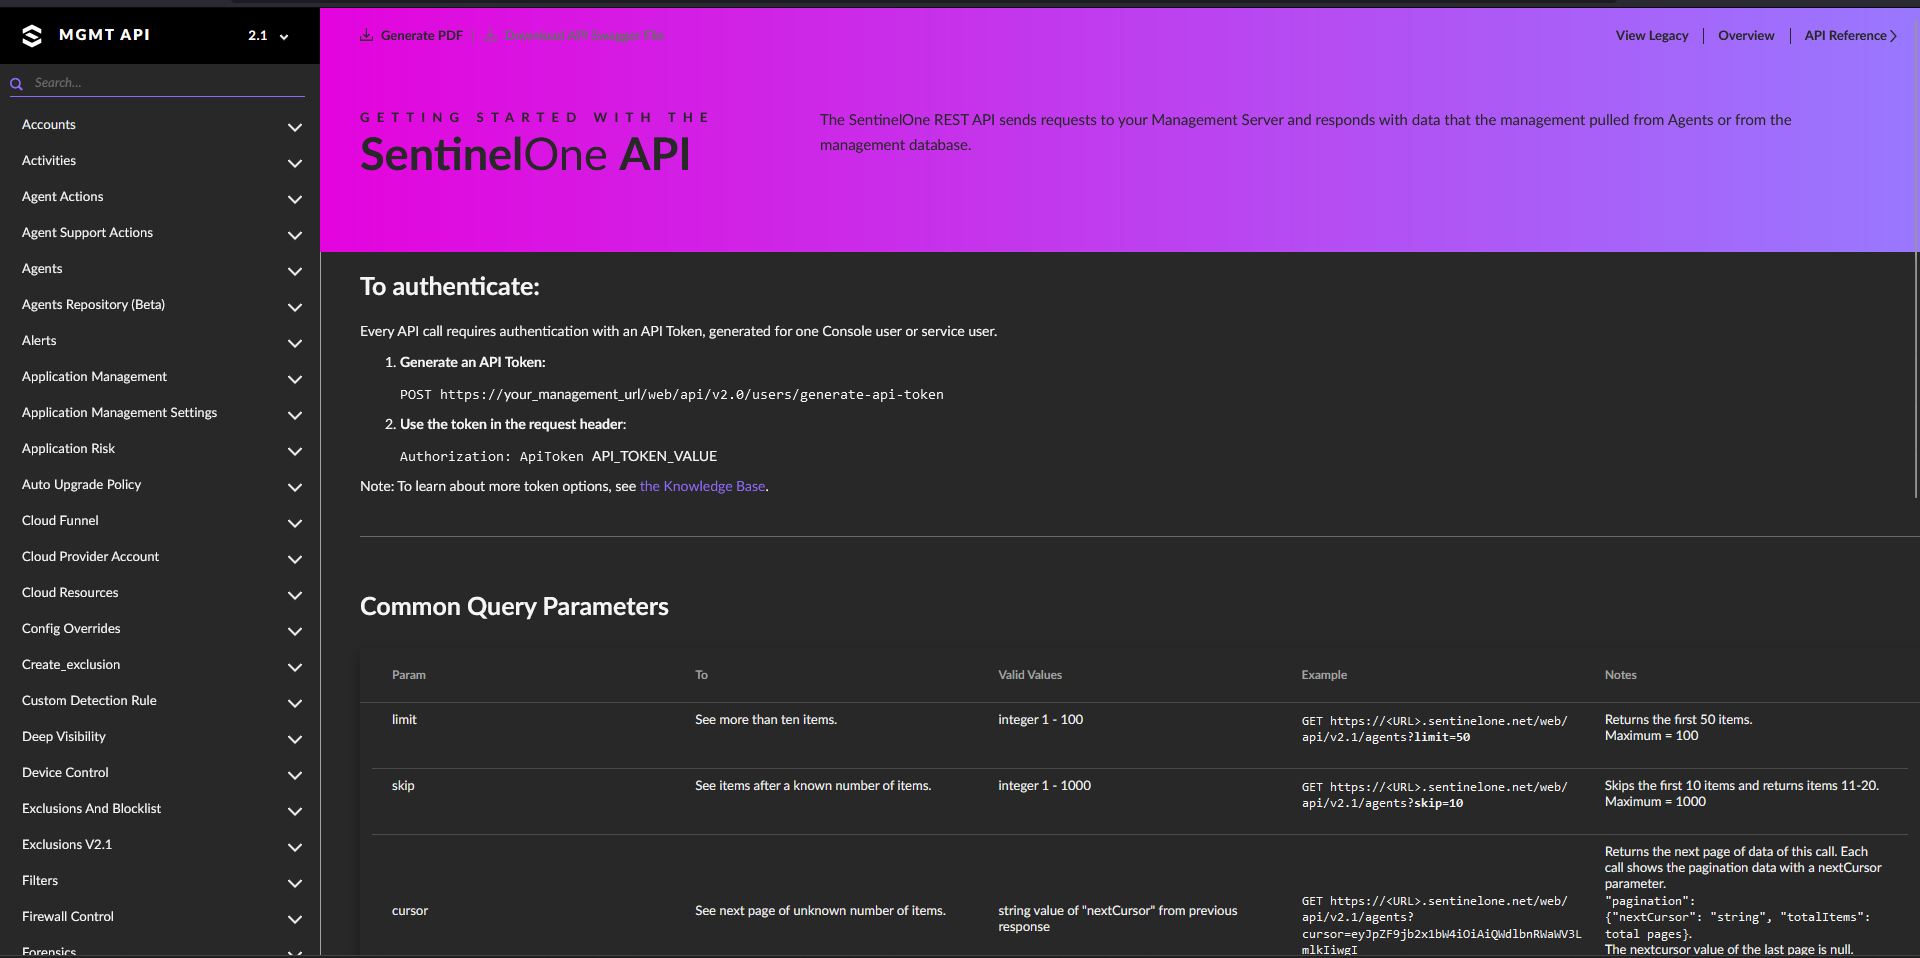
\includegraphics[width=0.8\textwidth]{Figures/SentinelOne/API Doc.png}
      \caption{SentinelOne API Documentation}
\end{figure}

\begin{multicols}{2}
      \section{Research Sub-Question \#4: What are the best data visualization techniques for SentinelOne?}
      Data visualization is the process of representing complex data (in the form of text and numbers) into a
      graphical representation, such as: interactive charts, dashboards, pie charts, and so on. In the context
      of this project, the displays should be able to tell interesting stories and share findings with diverse
      audience (the client, helpdesk, and cybersecurity analysts).

      \subsection{Data Visualization Widgets in Flutter}
      In Flutter, there are 3 famous library that supports a wide range of chart types,
      \href{https://pub.dev/packages/fl_chart}{fl\_chart},
      \href{https://pub.dev/packages/syncfusion_flutter_charts}{syncfusion\_flutter\_charts}, and
      \href{https://pub.dev/packages/flutter_echarts}{flutter\_echarts}. Each chart type is
      suitable for a specific kind of data and provides a different way to visualize the data. Types of charts in
      both libraries include 30+ plotting series:
      \begin{itemize}
            \item Line chart: is used to display data points connected by straight line segments. They are commonly
                  used to show trends over time.
            \item Bar chart: it uses rectangular bars to represent data. The length of each bar corresponds to the
                  value it represents. Bar charts are useful for comparing quantities of different categories.
            \item Pie chart: represents data in the form of slices of a pie. Each slice corresponds to a category
                  of the data, and the size of the slice is proportional to the quantity it represents.
            \item Scatter chart: uses dots to represent data points on a two-dimensional plane. They are useful
                  for showing the relationship between two variables.
            \item Radar chart: \acrshort{aka} spider chart or star chart, is a way of comparing multiple
                  quantitative variables. This makes them useful for seeing which variables have similar values
                  or if there are any outliers among each variable.
      \end{itemize}
\end{multicols}

\begin{figure}[htbp]
      \centering
      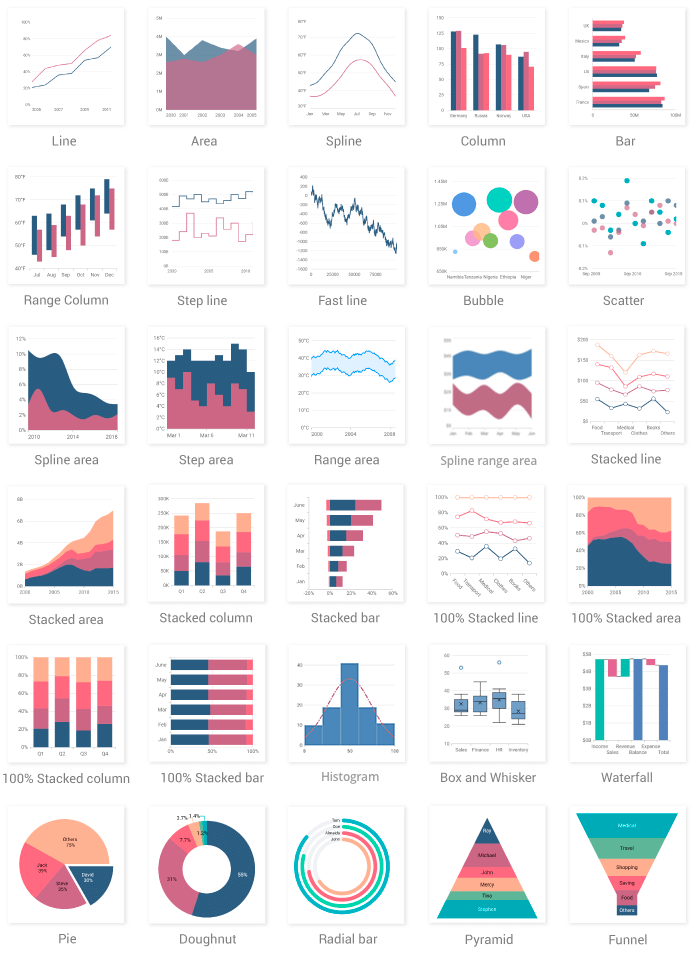
\includegraphics[width=0.8\textwidth]{Figures/Charts.png}
      \caption{Chart types in Flutter fl\_chart}
      \label{fig:charts}
\end{figure}

\begin{multicols}{2}
      Each chart type is easily configured with built-in support for creating stunning visual effects, and any
      number of series can be added to the chart. Features such as markers, data labels, data label builder,
      animation, gradient fill, dashes, sorting, and annotations are easy to incorporate and customize.

      Several main components of each chart type are:
      \begin{itemize}
            \item Chart data: the most important part is the data wanted to be displayed. This could be a simple
                  list of numbers, or more complex data structure, depending on the type of chart.
            \item Chart type: the second most important part is to specify the type of chart.
            \item Axes: the x and y-axes of the chart. The axes provide a reference frame for the data points and
                  can be customized to suit user's needs.
            \item Grid: the grid lines on the chart. These lines can help users better understand the data by
                  providing a reference frame.
            \item Touch response: the way the chart responds to user's touch events. It can be customized by
                  providing different types of interactivity, such as highlighting a data point when it is touched.
      \end{itemize}

      \textbf{Axis Types}

      Axis features such as label intersecting, edge label placement, label rotation, axis opposition, inverse
      axis, and multiple axis allow users to customize axis elements to make an axis more readable. Four of the
      axis types that are supported are:
      \begin{itemize}
            \item Numeric
            \item Category
            \item Date-time
            \item Logarithmic
      \end{itemize}

      \textbf{User Interaction}

      The package greatly enhance \acrshort{ux} by adding the following functionalities:
      \begin{itemize}
            \item Zooming and panning
            \item Crosshairs
            \item Trackballs
            \item Drilling down
            \item Events
            \item Selection
            \item Tooltips
      \end{itemize}

      \textbf{Legend}

      The package also supports legends, which display additional information about a chart series. The legends
      can be used to collapse the series and can be wrapped or scrolled if items exceed the available bounds.

      \subsection{Comparison to other EDR solutions}
      To determine the best visualization techniques for SentinelOne, a comparison to other \acrshort{edr}
      solutions is needed. In this section, the author has looked into other alternatives to SentinelOne, which are
      a single \acrshort{epp}/\acrshort{edr} solution, created as a complete replacement of legacy \acrshort{av}.
      Please keep in mind that in this sub-question, only the visualization techniques will be assessed, compared,
      contrasted, evaluated, and discussed. The other factors such as pricing, technologies, and features will not
      be discussed in this sub-question.

      \subsubsection{Heimdal\textregistered}

      On the homepage, information about each of the products/modules that are active under the current customer
      account is shown. The chart, which can be seen include a variety of Bar charts, Pie charts, and Line charts,
      include data regarding attacks, vulnerabilities, detections, infected/quarantined files, blocked/allowed
      processes, third-party application vulnerabilities or \acrshort{os} updates, and quarantined/rejected e-mails.

      \subsubsection{CrowdStrike}


      \subsubsection{Trend Micro} % Fukujima
      Trend Micro Apex One has customizable contents and layout of their dashboard. Workload Security uses Session
      to save user's settings and remember the last view of the dashboard the next time the user log in.
      The colour here is a bit basic with only the typical
      red, green, blue, and yellow.

      Based on the three examples above, some conclusion can be drawn about the techniques they use in their
      dashboard:

      \textbf{Visualization techniques}

      All three solutions use a combination and types of bar charts, pie charts, and line charts to display data.
      This due to the fact that the type of data they are trying to display is categorical and numerical data.
      Categorical data is data that can be divided into distinct groups or categories with no inherent order, and
      one category  can only have one value.

      Pie charts are used to visualize relative proportions or percentages of different categories within a
      dataset. Each category is represented by a slice of pie, with the size of each slice corresponding to the
      proportion of that category relative to the whole dataset.

      Bar graphs are used to compare the quantities or frequencies of different categories. Each category is
      represented by a separate bar, with the height (or length, in horizontal bar graphs) of the bar indicating
      the value of that category.

      In the case of SentinelOne integration to the \acrshort{qaas} app, both bar and pie charts can be used with
      the addition of line charts to display the timeline of a Threat Incident, and Scatter charts to show the
      relationship between two variables.

      \textbf{Customizable Widgets}

      All three solutions allow users to customize the layout and contents of their dashboards. This is important
      as different users may have different preferences and requirements for the data they want to see. Customizable
      widgets allow users to choose which data they want to display, how they want to display it, and where they
      want to display it on the dashboard.

      The SentinelOne dashboard of the \acrshort{qaas} app should have this functionality, therefore it should
      store user's preference
      \textbf{Coloring}

      \subsection{Conclusion}
      In Flutter, there are two main libraries that support a wide range of chart types, which are: fl\_chart and
      syncfusion\_flutter\_charts. Each chart type is suitable for a specific kind of data and provides a different
      way to visualize the data. The SentinelOne data will mainly be displayed by using pie chart and bar graph
      because the data is categorical and numerical. Comparing to the other \acrshort{edr} platform, the dashboard
      of the \acrshort{qaas} app should have customizable widgets, allowing users to choose which data they want
      to display, how they want to display it, and where they want to display it on the dashboard. The dashboard
      should also store user's preferences and settings, so that the user can see the same view the next time they
      log in. The colour of visualization charts should not be more than the typical red, green, blue, and yellow,
      as it can be overwhelming and confusing to the user. Red colour is usually used to indicate a problem or a
      threat,  green colour is used to indicate that everything is okay, while grey colour is used to indicate that
      the data is neutral or not critical, or that the data is not available. Different colours such as purple,
      blue, and yellow will also be used to indicate different categories of data. Additionally, the dashboard
      should also have a legend to display additional information about the chart series.
\end{multicols}